\documentclass[10pt,conference,compsocconf]{IEEEtran}

\usepackage{hyperref}
\usepackage{graphicx}	% For figure environment
\usepackage{bbm}


\begin{document}
\title{CS433-Machine Learning Project 1}

\author{
  Amaury Combes - Vincenzo Bazzucchi - Alexis Montavon\\
}

\maketitle

\begin{abstract}
  The Higgs Boson Kaggle challenge was put in place by physicists in CERN in order to analyze the massive data gathered during their research with the Large Hadron Collider. The idea was to use the best algorithms to predict if a particle collision event was a signal of the Higgs Boson. This challenge was actually one of the biggest ever on Kaggle and we reproduced it in our Machine Learning class at EPFL.
\end{abstract}

\section{Introduction}

TODO: at the end

\section{Model and Methods}
\label{sec:model}
\subsection{Preprocessing}
After diving into the dataset the first question that came to our attention was what to do with the undefined values \textit{-999.0}. Three options came to mind, setting them to 0, to the average of every valid values in each feature or to the most frequent value in each feature. We opted for the second option as it seemed more coherent than the first one (although there wasn't any clear differences on the final accuracy result) and it turn out to be better than the last one when we cross validated our model. This is done by the \textit{mean\_spec} function in the \textit{preprocessing.py} file.\\ We then decided to standardize the dataset to avoid too big variations in its values. We implemented a classic standardization function, see \textit{stadardize} function in the \textit{preprocessing.py} file.\\ As we saw in class, linear models are not very rich, so we used the polynomial augmentation technique used in the lab session. This is realized by the \textit{polynomial\_enhancement} function in the \textit{preprocessing.py} file.\\
Finally, on the advice of different TAs and the article \cite{anderson04}, we chose to train our model on each "categories" based on the numbers of jets (this is given by the column \textit{PRI\_jet\_num}). To do so we retrieve the indices of the rows belonging to the category, extract every row, delete the category indicator column and train on each category. This is done with the \textit{category\_iter} function in the \textit{run.py} file.

\subsection{Preparing the data for learning}
We performed the preparation of the data matrix before training. This consisted "applying" the degree of the model to the data: given the data matrix $D$, and the degree $d$ we obtained our matrix $X$ by concatenating a column of ones and the successive powers of $D$ : $$X = [\vec{1} | D | D^1 | D^2 | \dots | D^d]$$

\subsection{Models}
We implemented and compared different models, all of them are linear models. Therefore one of the parameter we had to tune was the degree of the model.

To compare our models we used k-fold cross validation and computed the \textit{accuracy}. Given the real classification $\vec{y}$ and the predictions we computed $\vec{p}$, both of length $n$ we can simply compute the accuracy $$a(\vec{y}, \vec{p}) = n^{-1}\sum_{i=1}^n \mathbbm{1}\{y_i = p_i\}$$

\subsubsection{Least squares}
Our first attempt consisted in implementing a simple least squares model. As the size of the matrix is relatively small and our machines could inverse it quite easily, we only tried to use the matrix inverse and the pseudo-inverse.

This means that given the data matrix $X$ and the prediction vector $\vec{y}$ we computed the weight vector $\vec{w}$ by
$\vec{w} = X^{-1} \vec{y}$. As the matrix was often singular, we used the pseudo-inverse: $X = U \Sigma V^T$ and then
$$\vec{w} = V \Sigma^{-1} U^T \vec{y}$$
We were surprised by this method as our very first attempt with least squares (with degree 1) gave us an accuracy of $0.744388$ with a 5-fold cross validation and we reached an accuracy of $0.807668$ when training the data enhanced to a degree 8 polynomial. 
Least squares is implemented in \textit{leastsquares.py}.\\
After this we tried to train the model on each different category as explained in the preprocessing part. The only remaining thing was to find the best degree for each category and we improved our score to $0.825183780696$. 

\subsubsection{Logistic regression} After learning in the lectures about classification, we implemented logistic regression. Given the matrix data, we compute the probability that the point $\vec{x}$ is in category 1 by $\sigma(\vec{x}^T\vec{w})$ where $\sigma(t) = e^t (e^t + 1)^{-1}$. We do so by iteratively minimizing the loss function
$$L(\vec{w}) = \sum^n_{i=1} \ln(1 + \exp{\vec{x}^T \vec{w}}) - y_n \vec{x}^T\vec{w}$$
As the gradient $\nabla L(\vec{w}) = X^T(\sigma(X\vec{w}) - y$ and the Hessian matrix $H_{L}(\vec{w}) = X^TSX$  (where $S_{nn} = \sigma(\vec{x}_n^T w)(1 - \sigma(\vec{x}_n^T\vec{w})$) of the loss function can be easily computed, we found our best results by using Newton's method for minimization which computes $$\vec{w}^{(t+1)} = \vec{w}^{(t)} - \gamma^{(t)} (H^{(t)})^{-1}\nabla L(\vec{w}^{(t)}$$

Logistic regression is implemented in \textit{logistic.py} and uses minimizers defined in \textit{minimizers.py}. Using this implementation of logistic regression we improved our accuracy to $0.81632$, testing it on a 5-fold cross validation with a degree 4 and the gamma parameter set to $0.1$. We trained this model on every different category, as we did for Least Squares, and again obtained a better score of $0.82685350422$.

\subsection{Parameter tuning}
To select the best parameters for our models (the degree of enhancement and the gamma of the newton method) we ran a grid search over the cross validation with a fair range for those parameters. We found out that the best degree for Least Square was 8 and 5 for the Logistic regression.
\begin{figure}[tbp]
  \centering
  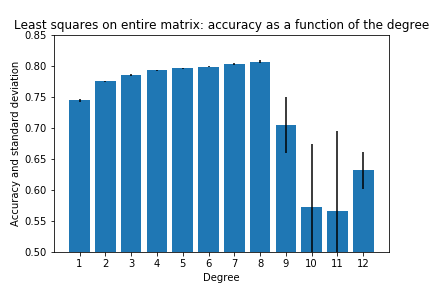
\includegraphics[width=\columnwidth]{ls_deg}
  \caption{Grid search on degrees for Least Squares on entire matrix.}
  \vspace{-3mm}
  \label{fig:denoise-fourier}
\end{figure}
\begin{figure}[tbp]
  \centering
  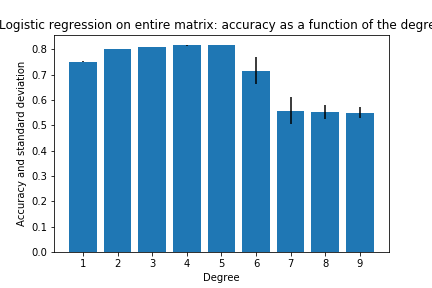
\includegraphics[width=\columnwidth]{lr_deg}
  \caption{Grid search on degrees for Logistic Regression on entire matrix.}
  \vspace{-3mm}
  \label{fig:denoise-fourier}
\end{figure}

\section{Results}

TODO: I guess best results we got and the exact techniques and parameters, give exact loss (mean of cross validation maybe)

\section{Summary}

TODO: Retrace best option we used in short

\bibliographystyle{IEEEtran}
\bibliography{literature}

\end{document}
